%\chapter*{Introduction}
\section{Problem Definition}

%\subsubsection{Motivation}
Blockchain transactions can be slow, sometimes taking hours to complete validation and verify integrity. Since a certain amount of work must be done to help prevent any abuse of the blockchain system and each block in the blockchain usually having a set limit for its transactions, scalability becomes an issue of blockchain. To help alleviate this issue, our idea is to create separate concurrent transaction chains that can handle transactions based on size, risk, and intention. For example, low risk transactions would be given priority to blocks that require less work to mine and therefore have a faster transaction rate. 

\section{How Blockchains Work}

A blockchain is a type of database that stores the information together in groups, which are called blocks. Each block has a certain capacity of storage for the information, therefore when it is filled, it will be closed and added to the end of the blockchain. This data structure of compiling the data into chunks and stringing them together creates an irreversible timeline of data and makes it a great way of storing data about all kinds of transaction histories. The most widely known use is for storing monetary transactions.

The goal of blockchain is to allow the information to be recorded and distributed, but not edited. Therefore, other than the data a user wants to store, each block also contains its own hash, which identifies the block, as well as the hash of the previous block, and the hashes of sequential blocks can be compared to ensure the integrity of the blockchain. The hash is usually created by a mathematical algorithm which uses the information stored in the block and turns it into a string. This process is one-way and irreversible. If the information is modified, the hash of a block should be different as well, further invalidating the rest of the blockchain. The most common hashing algorithm is SHA-256 which is being used for Bitcoin’s blockchain. However, with modern computers, hashes can be generated very fast and therefore, if a piece of information is being tampered with, the hash of the block which contains that information and the entire following blocks can be easily recalculated. To prevent that, blockchain uses Proof-of-Work mechanism to ensure that each block can only be created after satisfying some conditions, which would cost a certain amount of computing power. The computation process of creating a block is also called mining. In Bitcoin’s blockchain, it requires the hash of a block to begin with nineteen zeroes. And since the result of the hash function can not be influenced, computers will need to keep calculating until a hash that satisfies the condition comes up. This increases the difficulty of creating a block, as well as the cost of attempting to tamper with the data of an existing block.

\begin{figure}[!ht]
   \centering
   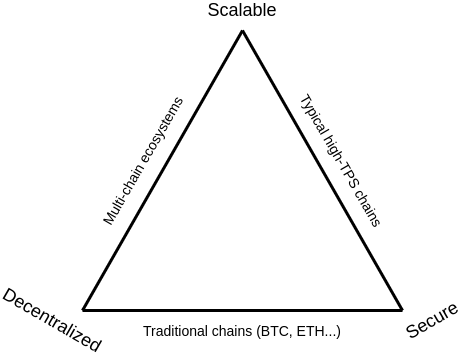
\includegraphics[width=120mm]{fig/trilemma.png}
   \caption{V2 Performance Chart}
\end{figure}

Blockchain also ensures its security by allowing the data in the database to be spread out among different network nodes in multiple locations. In other words, it decentralizes the data so that it won’t be easily tampered with. In the case of false information being stored, blockchain uses a fault-tolerant mechanism called consensus mechanism 
which requires the consensus of a majority of the network in order to modify the content of a block.

\section{Challenges of Traditional Blockchains}

Most blockchains depend on a proof-of-work consensus mechanism for validating transactions. This works by machines competing with each other to generate a hash that usually begins with a specified number of zeros. Each block gets processed one at a time and must be consistent with the rest of the blockchain. Such an approach works fine for a limited number of transactions. But as the transaction rate increases over time, the approach struggles to scale to meet demand. For example, Visa — a famous payment provider, has a non-blockchain network that achieves an throughput of 1700 transactions per second (TPS), whereas Bitcoin only maintains an average of 7 TPS. This issue with scalability is one of the biggest issues that modern blockchain implementations are facing. Currently, several popular cryptocurrencies such as Ethereum are in the process of researching a solution for this exact problem.

\section{Benefits of Parallelizing Blockchain}

Blockchain technology is a serial data structure, where each block must be processed one by one. This limits the speed of the technology because transactions occur mostly sequentially. Parallel processing is a very effective technique used to solve large-scale problems, in the case of blockchain, this would mean unrelated transactions could occur concurrently which would yield more confirmations at a time. 
There are risks and costs associated with every technology, and with proof-of-work blockchains, we see a generally high computational power need. Ethereum, one of the largest cryptocurrencies in the world, uses around 113 terawatt-hours per year- the equivalent to about as much energy as the average US household uses in one week used for every single transaction. With the mechanism only being able to handle 15 transactions per second, it’s also slow. Additionally, cryptocurrencies relying on a proof-of-work system are inherently difficult to scale.

Proof-of-stake systems are more performant due to its preference in capital over computing power, and being more compatible with parallel processing. This allows us to employ the help of a technique known as sharding. Sharding helps enable faster throughput by splitting a blockchain into several different instances that run in parallel. These shard chains increase the transactions per second rate since executions won’t occur sequentially. With a parallel blockchain, one can expect the energy problem associated with proof-of-work to decrease substantially and transaction speed to soar. It lessens the environmental impact that proof-of-work has, but of course has its own risks and costs.

\section{Researching a Viable Solution}

Before working on this project, our group had little understanding as to how blockchain actually worked. This led to a constant need of research and experimentation throughout the course of this project. As it turns out, not all blockchains are built the same even though they may appear similar on the surface. These differences resulted in difficulties as we progressed through the project as some so called "solutions" that we found and attempted to implement needed to be scrapped due to the contrasts in structure.

Eventually we became interested in developing a bare-bones prototype that is similar to what Ethereum is planning with their upcoming Ethereum 2.0 release. This led us to reading and referencing several papers written by Vitalik Buterin, who is the founder and leader of the Ethereum 2.0 project. These papers are detailed and explain the theory of Proof-of-Stake, Shard Chains, and the Beacon chain very well. All that was left was to tweak the process to our specifications and implement these ideas into our programs.

\section{Implementation}

We will be implementing our solution with the Java programming language. While not as performant as a language such as C++, Java is better suited for the rapid prototyping of our proposed design.

Since we plan to experiment throughout the project, we will be storing our experiments as different versions of the project. This will allow us to reference these versions and draw comparisons between them as needed.
Additionally, we will be writing Unit Tests to ensure that future changes to the project do not result in invalid output or break the project.

The different versions of the project are as follows:
  \begin{itemize}
    \item Version 1 — Proof of Work
    \item Version 2 — Proof of Stake
    \item Version 3 — Proof of Stake with Sharding
  \end{itemize}
 

\section{Consensus Mechanisms}

\subsubsection{Proof-of-Work}

Proof-of-work is the original crypto consensus mechanism, which was first used by Bitcoin. The idea behind this consensus is that the blockchains are secured and verified by virtual miners around the world which are racing to be first to solve a “math puzzle.” The solution to this puzzle requires a certain amount (typically being large) of computational power. The winner gets to update the blockchain with the latest transaction and is then rewarded by the network with a predetermined amount of crypto. This consensus mechanism has its advantages, such as the fact that it is a proven, robust way of maintaining a secure decentralized blockchain. As the value of the cryptocurrency increases, more miners are incentivized to join the network, which in turn increases the power and security of the blockchain. However, it also has its disadvantages. Because Proof-of-Work can become very energy-intensive considering such a large amount of transactions that can occur, it does not scale very well to accommodate that. Another flaw is a security issue. If a sub-blockchain within the network becomes bigger than the main blockchain, it will replace it. This is extremely unlikely to happen, especially for larger cryptocurrencies, but for smaller ones it can happen. This can pose a serious security issue.

\subsubsection{Proof-of-Stake}

The developers of the Proof-of-Stake consensus mechanism knew from the beginning that the Proof-of-Work mechanism would post limitations in scalability that would eventually need a solution to. This is  why Ethereum is investing so many resources into making the conversion for Ethereum 2.0. In a Proof-of-Stake system, “staking” is different from the Proof-of-Work’s “mining,” in that it’s the process by which a network participant gets selected to add a batch of transactions to the blockchain and earn some amount of crypto in exchange, instead of all machines competing for a single block in an arms race. Instead of having a math puzzle to solve, a “validator” can contribute, or stake, their own crypto in exchange for a chance of getting to validate a new transaction, update the blockchain, and earn a reward. The whole process can be summarized in three steps:
  \begin{enumerate}
    \item The network selects a winner based on the amount of crypto that each validator has in the pool and the length of time it has been there. (rewarding the most invested participant) 
    
    \item Once the winner has validated the latest block of transactions, other validators can then come in and verify that the block is accurate, and once a threshold number of those attestations has been met, the network updates the blockchain.
    
    \item All participating validators receive a reward in the native crypto, which is generally distributed in proportion to each validator’s stake. 
    
  \end{enumerate}	

Not everyone can become a validator. It is a major responsibility and requires a fairly high level of technical knowledge. The minimum amount of crypto that is required to stake is typically relatively high, and users can lose their stake if their node goes offline or if they validate a “bad” block of transactions. 

Proof-of-Stake can pose a disadvantage, however. A threat to this consensus mechanism is known as the 51\% attack. When a validator controls 51\% of a cryptocurrency, they can potentially have the ability to alter the blockchain. It is very expensive for someone to own 51\% of the staked cryptocurrency, however, so this is not common at all. Additionally, if foul play were to be detected, they would lose their stake. While unlikely to happen, this is still important to note as a potential security issue.

\section{Parallel Execution Model}

For this project, we will be attempting to design our own parallel execution model for blockchain. Currently, most cryptocurrencies rely on a linear execution model which struggles with scalability and provides very limited throughput for transactions. While a linear execution model may be used for smaller cryptocurrencies, it is no longer a feasible solution for the larger and more active ones.

To support parallel execution, we will be making use of the Proof-of-Stake consensus mechanism. Due to its nature, as previously defined, it is much more compatible with parallelism than the Proof-of-Work consensus mechanism. Additionally, we will be making use of a distributed network of nodes known as shards in a process called sharding. Such a design would allow our cryptocurrency to scale as needed.

\section{Sharding}

Sharding is a parallelization method that can help blockchains improve their efficiency and scalability–a big issue faced with blockchains. Sharding involves dividing an entire network into smaller partitions called shards. Each shard only needs to work on transactions relevant to their own. Different shards therefore can work in parallel to share the workload. The more shards there are, the better the performance.

\section{Performance Metrics}

As mentioned previously—we will be keeping track of multiple versions of the project. This is done to ensure that progress is being made as the project develops as well as allow us to compare performance and functionality between implementations.

\begin{figure}[!ht]
   \centering
   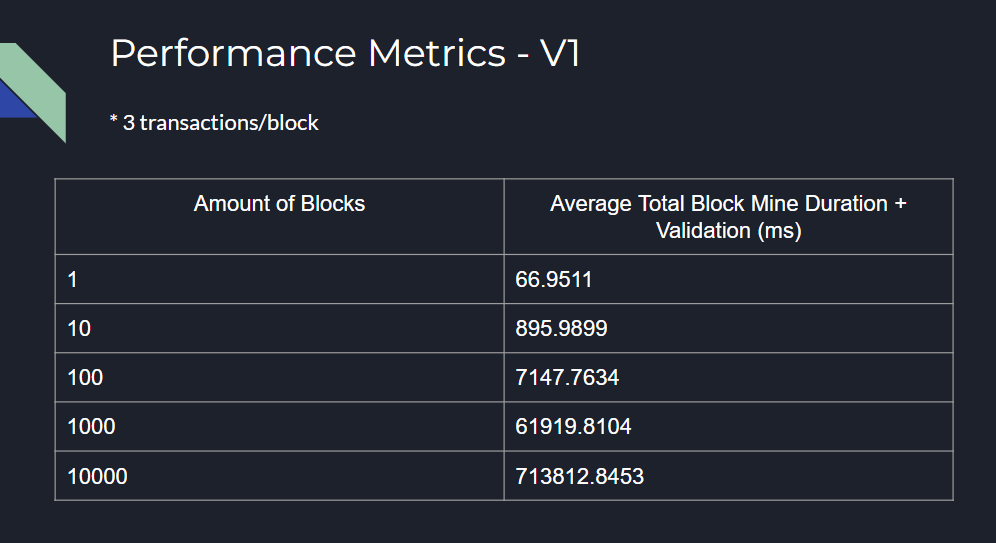
\includegraphics[width=120mm]{fig/V1.PNG}
   \caption{V1 Performance Chart}
\end{figure}

\begin{figure}[!ht]
   \centering
   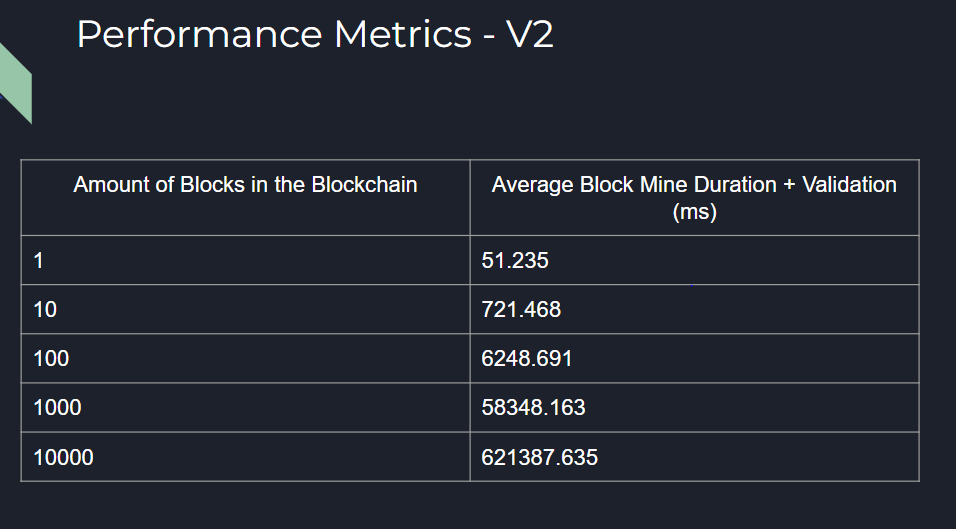
\includegraphics[width=120mm]{fig/V2.PNG}
   \caption{V2 Performance Chart}
\end{figure}

\begin{figure}[!ht]
   \centering
   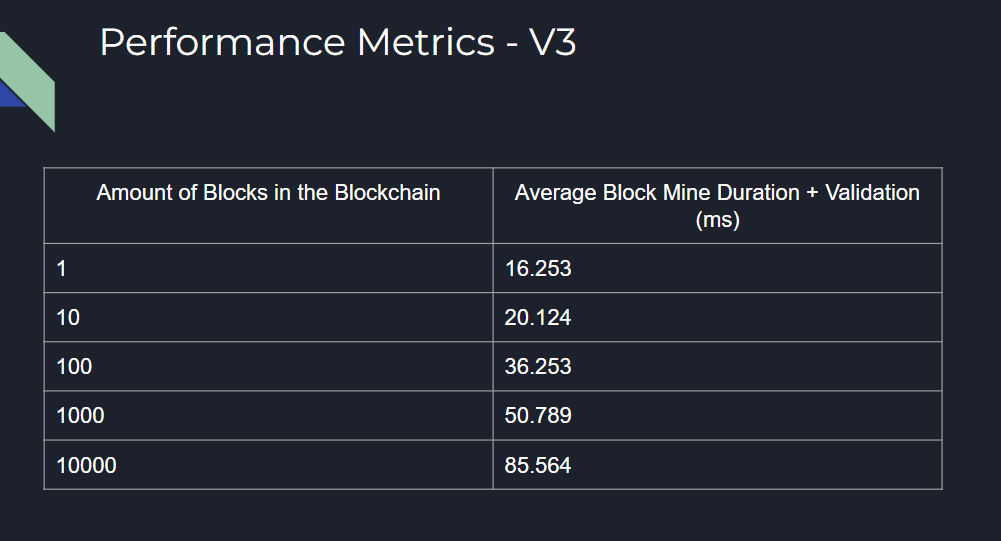
\includegraphics[width=120mm]{fig/V3.PNG}
   \caption{V3 Performance Chart}
\end{figure}

\section{Conclusion}
In conclusion, our theory implementing parallel concepts onto a Blockchain was successful. Apart from learning all about how Blockchains work, and their consensus mechanisms, we were also able to see a visible difference in performance. The efficiency in which the Blockchain was able to mine blocks and process transactions was dramatically increased through the use of concurrency and parallelism. This was of course done while also keeping the chain secure and validated.

~\nocite{frankenfield_2022}
~\nocite{ethereum.org}
~\nocite{adittane_2021}
~\nocite{bitpanda}
~\nocite{mearian_2019}
~\nocite{changelly.com_2021}
~\nocite{vitaliks}
~\nocite{changelly.com_2020}
~\nocite{ethereum.org2}
~\nocite{ethereum.org3}


% Used for inline citation
%\cite{book}


